\documentclass{article}
\usepackage{geometry}
\geometry{
a4paper,
total={254mm,254mm},
left=25mm,
right=25mm,
top=25mm,
}
\usepackage[spanish,mexico]{babel}
\usepackage[utf8]{inputenc}
\usepackage[T1]{fontenc}
\usepackage{imakeidx}
\usepackage{url}
\usepackage{hyperref}
\usepackage{graphicx}
\usepackage{float}
\usepackage{listings}
\usepackage{color}
\definecolor{mygreen}{rgb}{0,0.6,0}
\definecolor{mygray}{rgb}{0.5,0.5,0.5}
\definecolor{mymauve}{rgb}{0.58,0,0.82}
\usepackage{caption}
\usepackage{subcaption}


\lstset{ 
  backgroundcolor=\color{white},
  basicstyle=\footnotesize,
  breakatwhitespace=false,
  breaklines=true,                 % sets automatic line breaking
  captionpos=b,                    % sets the caption-position to bottom
  commentstyle=\color{mygreen},    % comment style
  deletekeywords={...},            % if you want to delete keywords from the given language
  escapeinside={\%*}{*)},          % if you want to add LaTeX within your code
  extendedchars=true,              % lets you use non-ASCII characters; for 8-bits encodings only, does not work with UTF-8
  firstnumber=1,                % start line enumeration with line 1000
  frame=single,	                   % adds a frame around the code
  keepspaces=true,                 % keeps spaces in text, useful fodõr keeping indentation of code (possibly needs columns=flexible)
  keywordstyle=\color{blue},       % keyword style
  language=c,                 % the language of the code
  morekeywords={*,...},            % if you want to add more keywords to the set
  numbers=left,                    % where to put the line-numbers; possible values are (none, left, right)
  numbersep=5pt,                   % how far the line-numbers are from the code
  numberstyle=\tiny\color{mygray}, % the style that is used for the line-numbers
  rulecolor=\color{black},         % if not set, the frame-color may be changed on line-breaks within not-black text (e.g. comments (green here))
  showspaces=false,                % show spaces everywhere adding particular underscores; it overrides 'showstringspaces'
  showstringspaces=false,          % underline spaces within strings only
  showtabs=false,                  % show tabs within strings adding particular underscores
  stepnumber=1,                    % the step between two line-numbers. If it's 1, each line will be numbered
  stringstyle=\color{mymauve},     % string literal style
  tabsize=2,	                   % sets default tabsize to 2 spaces
  title=\lstname
}


\begin{document}

\begin{titlepage}

\newcommand{\HRule}{\rule{\linewidth}{0.5mm}}

\center 

\textsc{\LARGE Universidad Nacional de San Agustín}\\[0.5cm]
\textsc{\LARGE Facultad de Ingeniería de Producción y Servicios}\\[0.5cm]
\textsc{\LARGE Escuela Profesional de Ciencia de la Computación}\\[1cm] 

\includegraphics[scale=0.85]{unsa-logo.png}\hspace{1cm}
\includegraphics[scale=0.3]{cs.png}\\[1cm]
\textsc{\LARGE{Física Computacional}}\\[0.3cm] 
\textsc{\LARGE{Práctica 6}}\\[0.3cm] 


\HRule \\[0.3cm]
{\huge \bfseries Ecuación de Onda}\\[0.3cm]
\HRule \\[0.3cm]

\begin{minipage}{0.7\textwidth}
    \begin{flushleft} 
        \Large{\textbf{Alumno:}}\\[0.3cm]
        {\Large{Cueva Flores, Jonathan}}\\[0.5cm]
        \Large{\textbf{Profesor:}}\\[0.3cm]
    {\LARGE{Llamoca Requena, Edwin}}\\[0.5cm]
    \end{flushleft}

\end{minipage}\\[1cm]

{\Large Arequipa - Perú}\\[1.2cm] 
\vfill 
{\Large Enlace donde se encuentra el proyecto en latex y la salida gif}
{\Large \url{https://github.com/tigerofmurder/p7-fisica}}
\end{titlepage}
\section{Solución aproximada de la ecuación de Onda}
\subsection{Analice el mismo problema, cambiando h y k y verifique sus resultados}
\begin{lstlisting}[language=Octave, caption=Código base de la ecuacion de la onda,label=lst:ondaFirst]
function U=onda(f,g,a,b,v,h,k)
% f es la condicion inicial de la posicion
% g es la condicion inicial de la velocidad
% v es la velocidad de propagacion de la onda
% a es la longitud de la cuerda
% b es la tiempo que se necesita para evaluar la onda
% h es la tama~no de paso para el espacio
% k es la tama~no de paso para el tiempo
% U es la matriz donde se almacena la solucion numerica
n=a/h+1;
m=b/k+1;
% r es calculo para la condicion de estabilidad
r=v*k/h;
r1=r^2;
r2=r^2/2;
s1=1-r^2;
s2=2*(1-r^2);
U=zeros(n,m);
% calculo de las primeras dos filas
for i=2:n-1
  U(i,1)=feval(f,h*(i-1));
  U(i,2)=s1*feval(f,h*(i-1))+k*feval(g,h*(i-1))+r2*(feval(f,h*i)+feval(f,h*(i-2)));
end
% calculo a partir de la tercera fila
for j=2:m-1
  for i=2:n-1
    U(i,j+1)= s2*U(i,j)+r1*(U(i-1,j)+U(i+1,j))-U(i,j-1);
  end
  surf(U)
end
\end{lstlisting}
\begin{figure}[H]
    \centering
    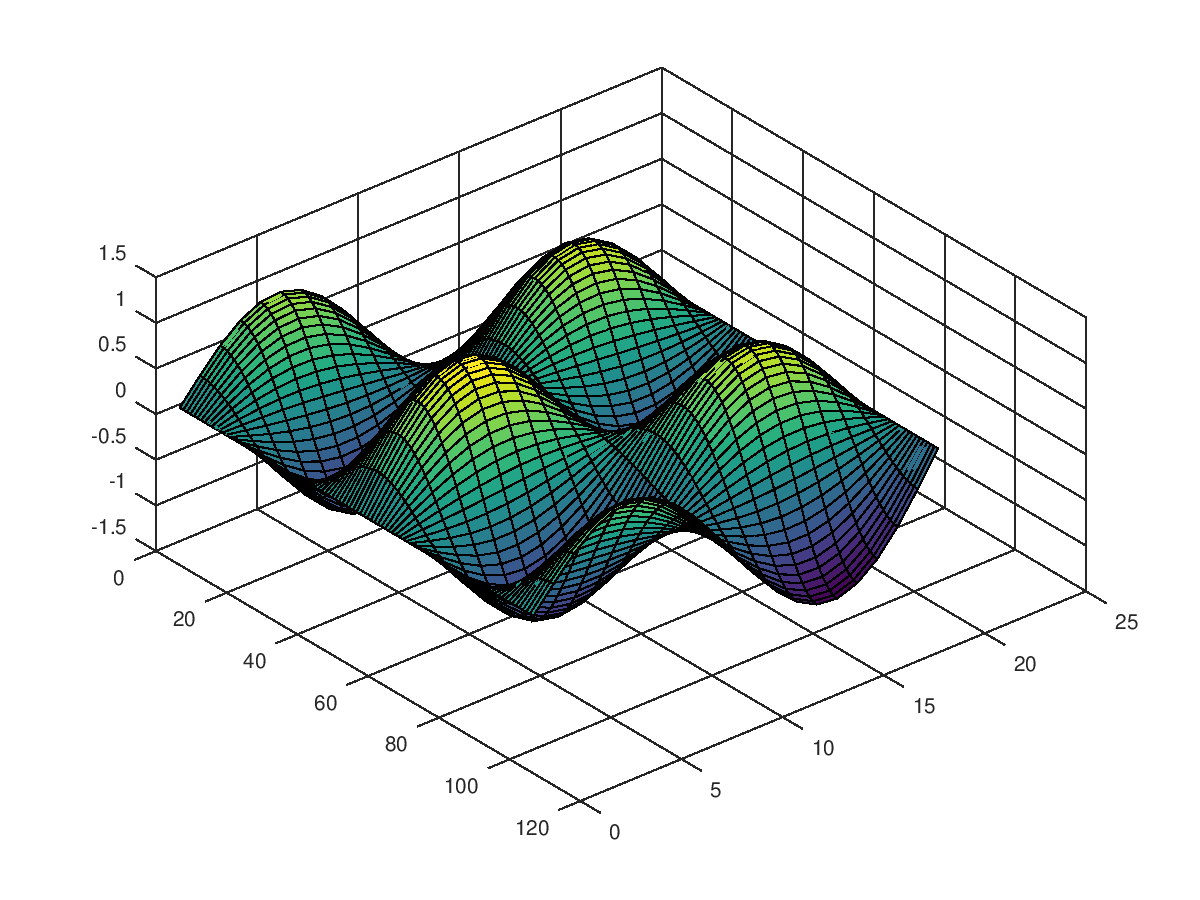
\includegraphics[scale=0.7]{1_1.png}
    \caption{h = 0.05 y k = 0.01}
    \label{fig:Solucion Real}
\end{figure}
\begin{figure}[H]
    \centering
    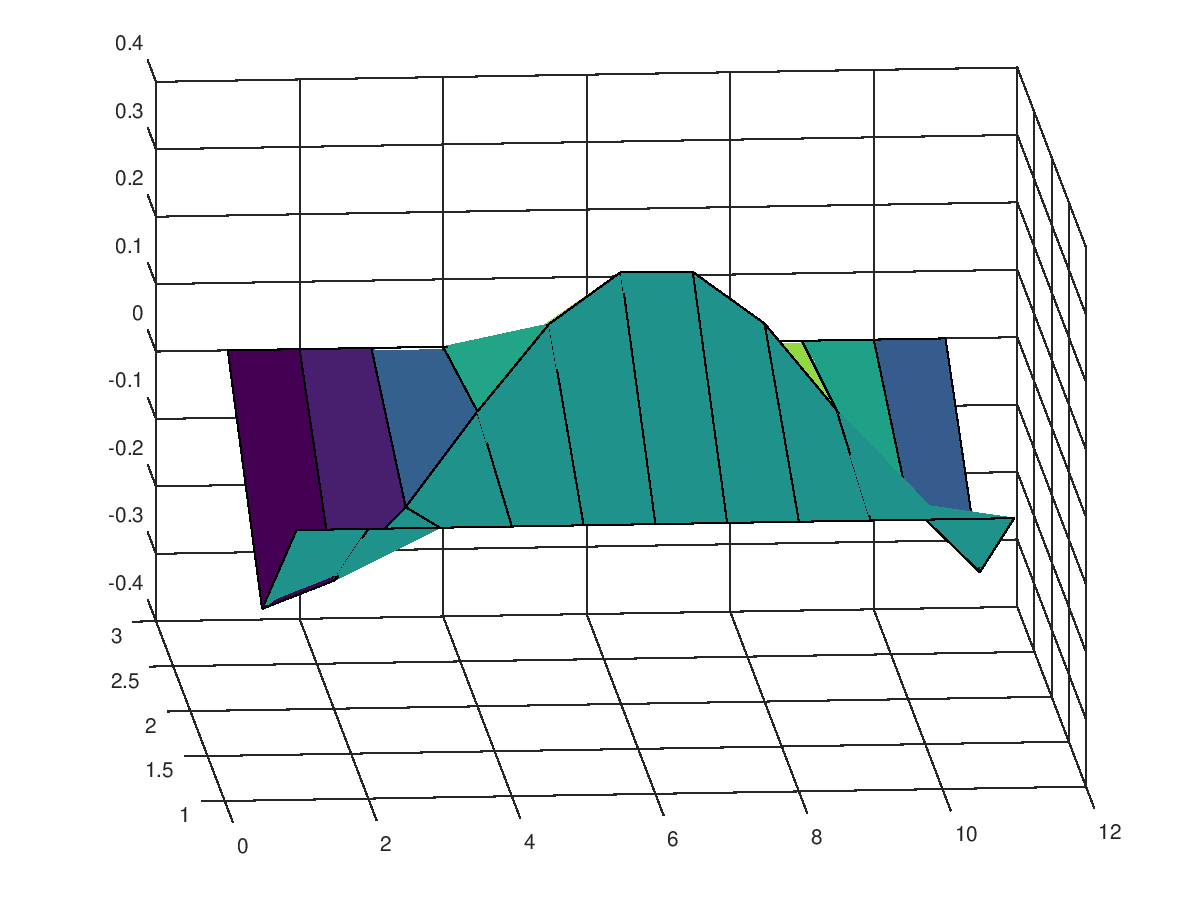
\includegraphics[scale=0.5]{1_2.png}
    \caption{h = 0.5 y k = 0.1}
    \label{fig:Solucion Real}
\end{figure}
\begin{figure}[H]
    \centering
    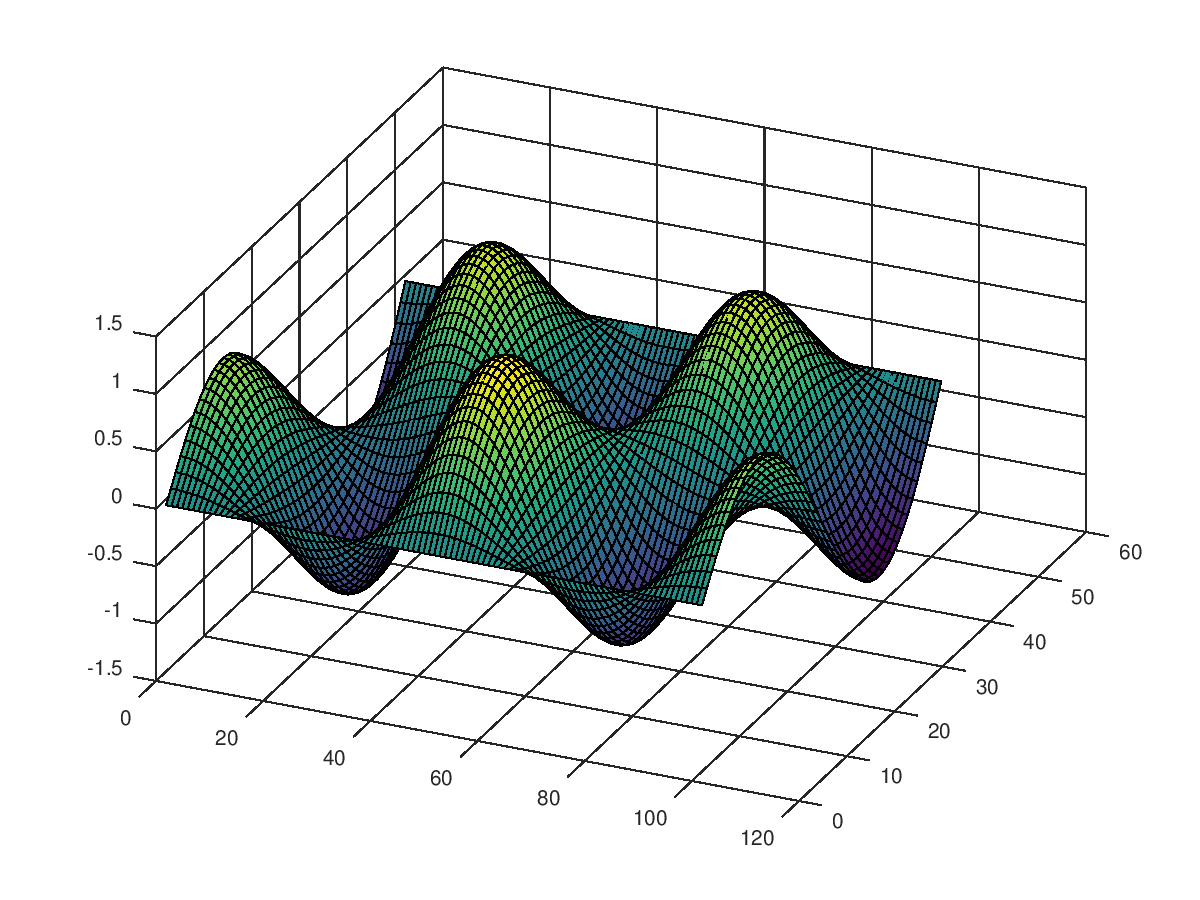
\includegraphics[scale=0.5]{1_3.png}
    \caption{h = 0.02 y k = 0.01}
    \label{fig:Solucion Real}
\end{figure}
Como conclusión tenemos que los valores h y k sirven para calcular r de esta forma mientras k se mas pequeño la simulación es mas fina.
\subsection{Verifique que si no cumple $r \leq 1$, como se verán los resultados ?}
Para comprobar el valor de $r\leq q$ disminuimos los valores k y h y aumentamos el valor v, entonces para este experimento se uso un h=0.4, k=0.1 y v=5 entonces para verificar que este sea mayor que 1 hacemos el calculo $r = v*k/h$ y se obtiene 1.25.
\begin{lstlisting}[language=Octave, caption=Comando y código de funciones g(x) y f(x) ,label=lst:]
function y = fx(x)
  y=x^2-x+sin(2*pi*x);
endfunction

function y = g(a)
  y=0;
endfunction

octave>>onda('fx','g',2,2,5,0.4,0.1)
\end{lstlisting}
\begin{figure}[H]
    \centering
    \begin{subfigure}[b]{0.9\textwidth}
        \centering
        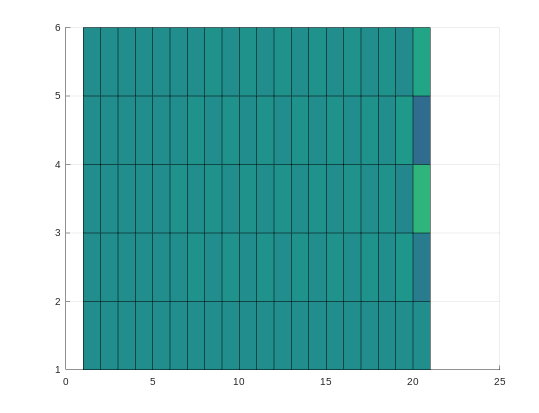
\includegraphics[width=\textwidth]{1.1.png}
        \caption{Mostrado en 2 dimensiones}
        \label{fig:XY}
    \end{subfigure}
    \begin{subfigure}[b]{0.9\textwidth}
        \centering
        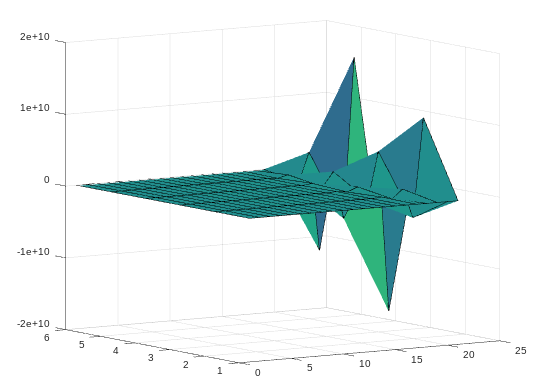
\includegraphics[width=\textwidth]{1.2.png}
        \caption{Mostrado en 3 dimensiones}
        \label{fig:XYZ}
    \end{subfigure}
    \caption{Resultados obtenidos utilizando los elementos que se presentaron al comienzo de la sección estos se muestran en la \ref{fig:XY} y \ref{fig:XYZ}.}
    \label{fig:SolucionR}
\end{figure}

\section{Problema desafió}
\subsection{Use a = 1, b = 1, v = 1, g(x) = 0}
\begin{equation}
    f(x)=  \left\lbrace
    \begin{array}{ll}
2x & \textup{si } 0\leq x\leq 1/2 \\
2-2x & \textup{si } 1/2 \leq x \leq 1
\end{array}
\right.
\end{equation}
Para este ejercicio se modifico la función f(x) para obtener el resultado esperado.
\begin{lstlisting}[language=Octave, caption=Funcion f(x) modificada para cumplir las condiciones que se pide,label=lst:fxMod]
function y = fx1(x)
  if 0<=x && x<=1/2
    y=2*x;
  elseif 1/2<=x && x<=1
    y=2-(2*x);
  endif
endfunction
\end{lstlisting}
\begin{figure}[H]
    \centering
    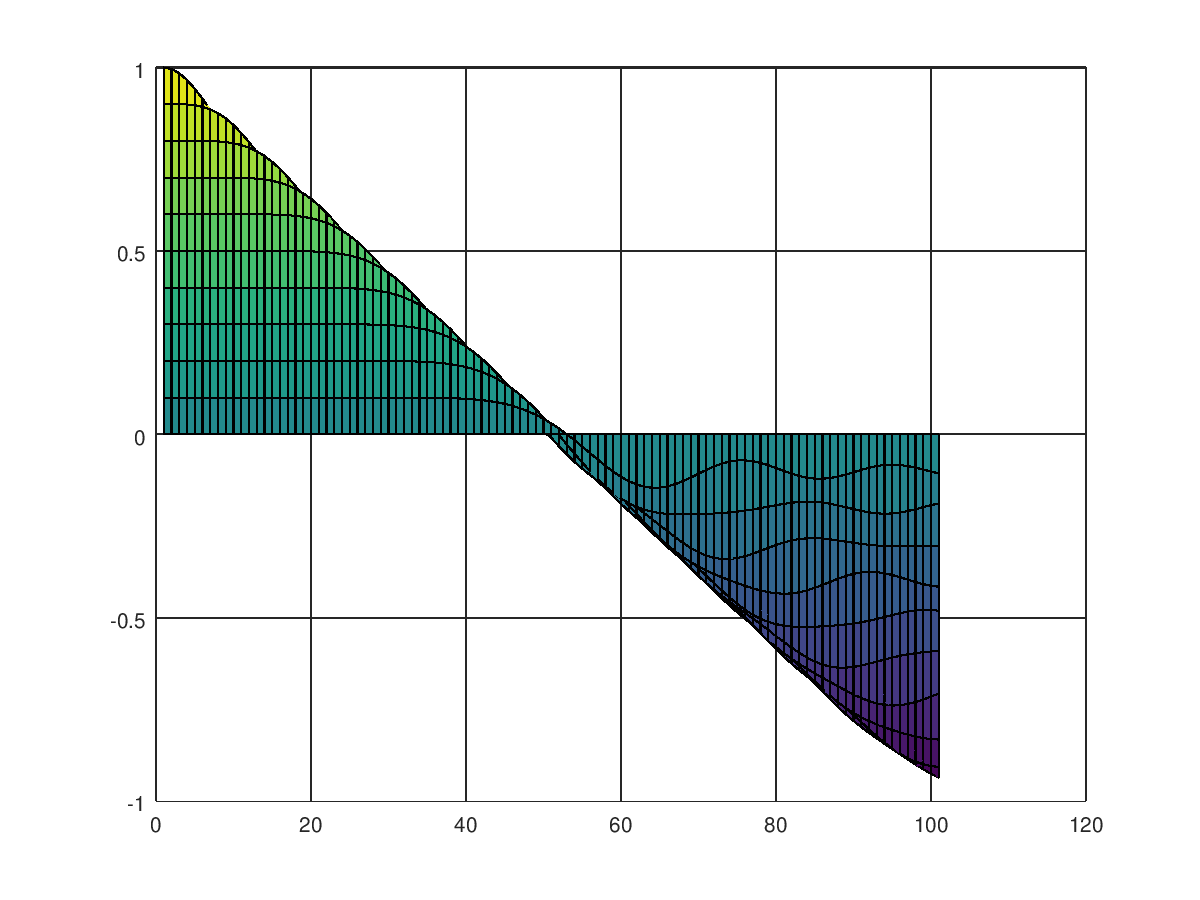
\includegraphics[scale=0.8]{3.1.png}
    \caption{Imagen mostrada de un ángulo lateral}
\end{figure}
\begin{figure}[H]
    \centering
    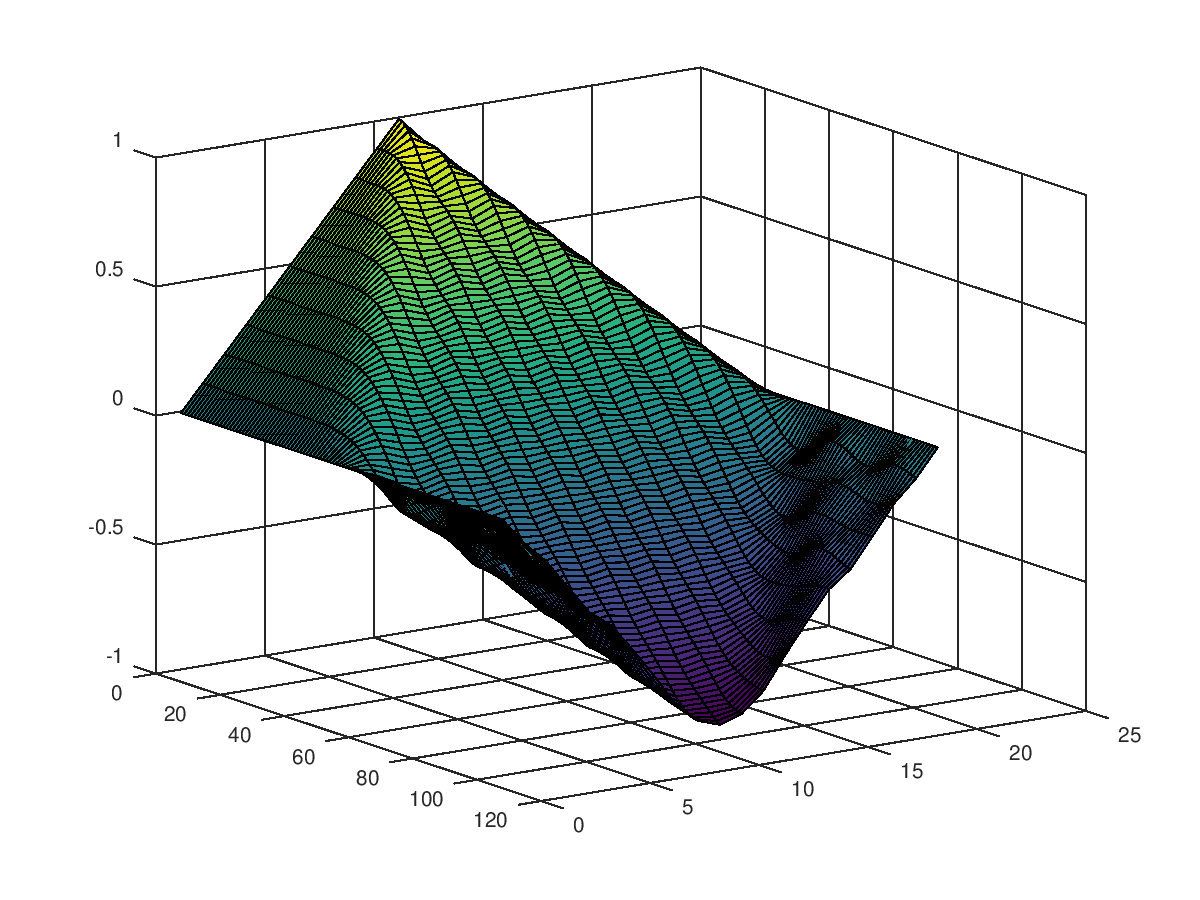
\includegraphics[scale=0.7]{3.2.png}
    \caption{Imagen mostrada con un ángulo de giro opcional para apreciar mejor la gráfica}
\end{figure}
\begin{figure}[H]
    \centering
    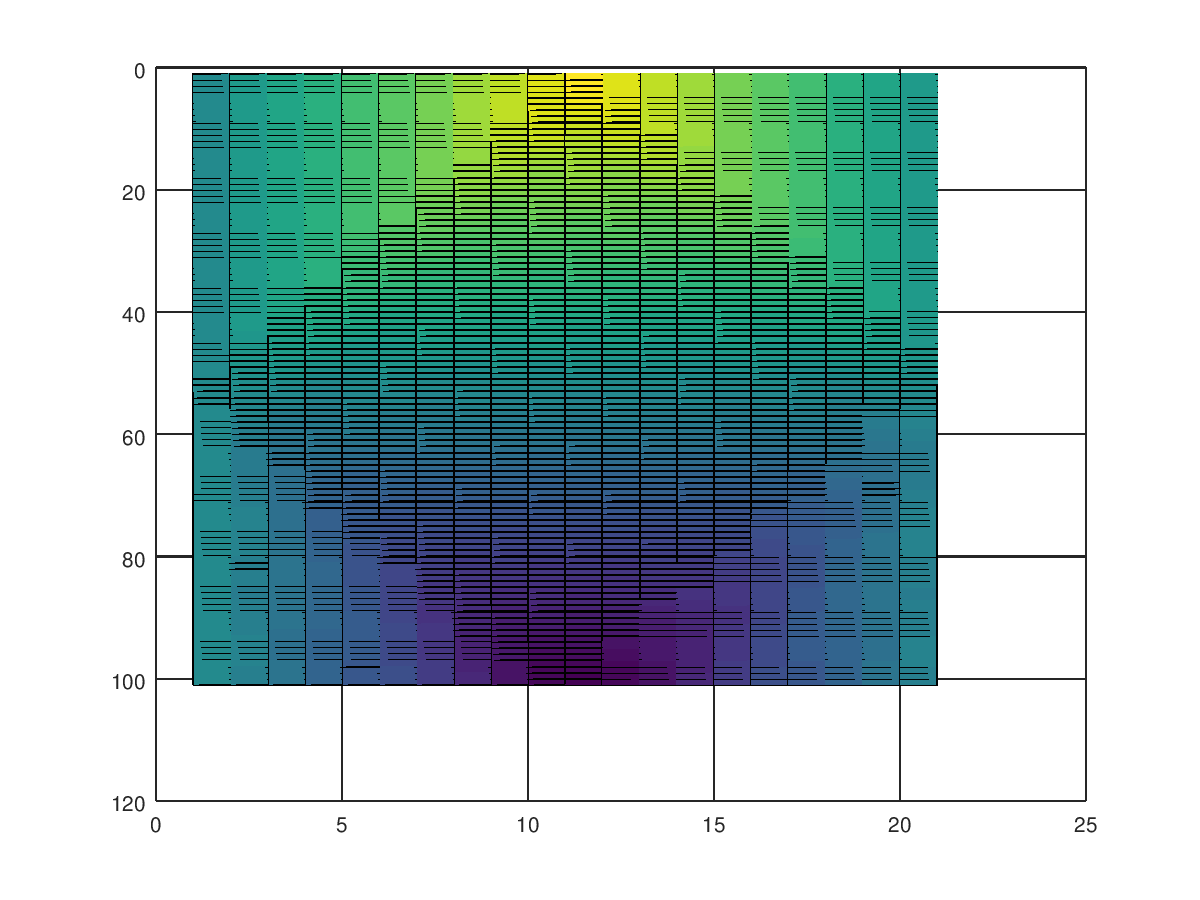
\includegraphics[scale=0.7]{3.3.png}
    \caption{Imagen mostrando desde la parte superior donde se ubica el espacio y el tiempo.}
\end{figure}
\begin{figure}[H]
    \centering
    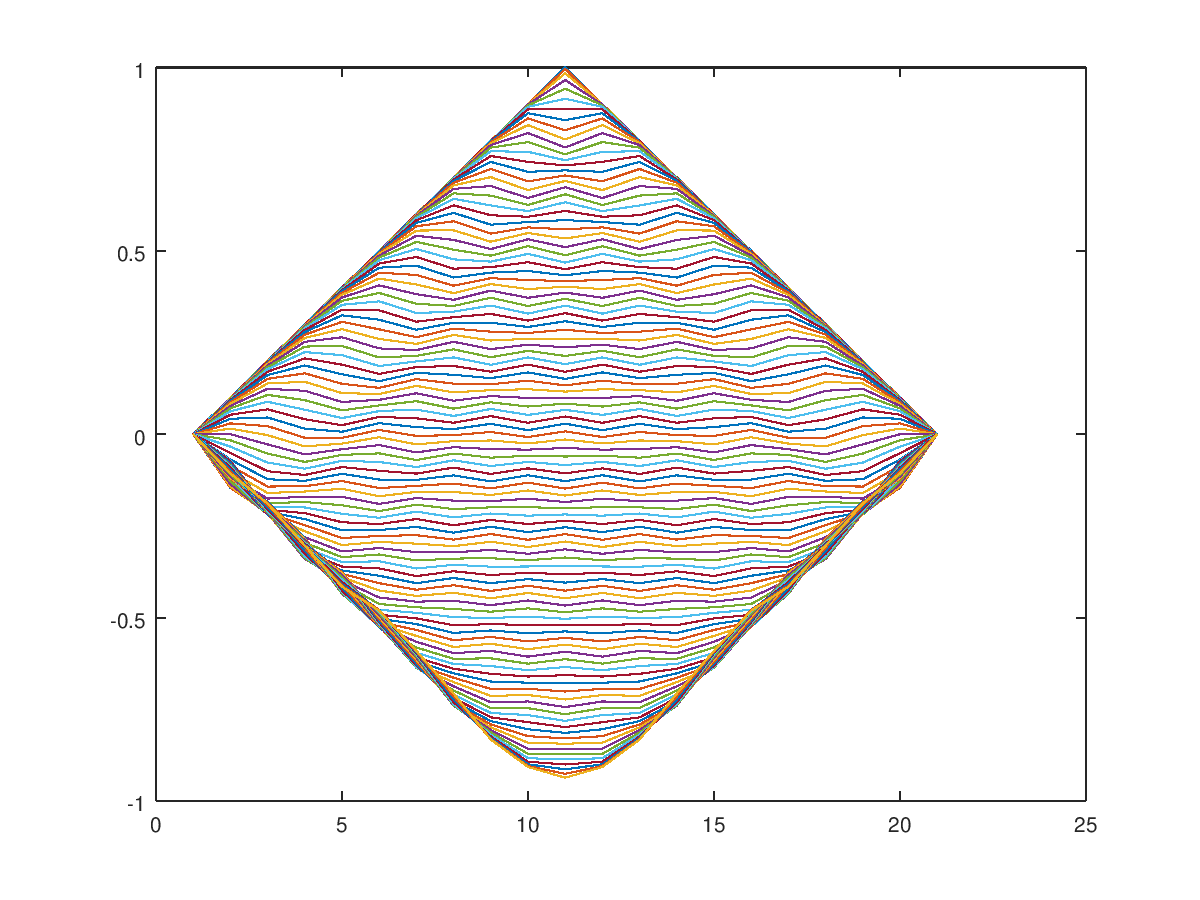
\includegraphics[scale=0.7]{3.4.png}
    \caption{Salida usando el comando plot con h = 0.05 y k =0.01}
\end{figure}

\subsection{Haga una secuencia de evolución paso a paso y que se grafique en forma independiente, ejemplo,utilice la instrucción subplot(10,10,x). Subplot(10,10,1) para j=1, Subplot(10,10,2) para j=2,etc.}
\begin{lstlisting}[language=Octave, caption=Version modificada del código para obtener el paso a paso de la gráfica,label=lst:lst_mods]
function U=onda(f,g,a,b,v,h,k)
n=a/h+1;
m=b/k+1;
% r es calculo para la condicion de estabilidad
r=v*k/h;
r1=r^2;
r2=r^2/2;
s1=1-r^2;
s2=2*(1-r^2);
U=zeros(n,m);
U_1=zeros(n,m);
% calculo de las primeras dos filas
for i=2:n-1
  U(i,1)=feval(f,h*(i-1));
  U(i,2)=s1*feval(f,h*(i-1))+k*feval(g,h*(i-1))+r2*(feval(f,h*i)+feval(f,h*(i-2)));
end
% calculo a partir de la tercera fila
for j=2:m-1
  for i=2:n-1
    U(i,j+1)= s2*U(i,j)+r1*(U(i-1,j)+U(i+1,j))-U(i,j-1);
  end
  if mod(j,3) == 0 
    subplot(10,10,j)
    plot(U-U_1)
    ylim([-1 1])
    pause(0.1)
  endif
  U_1 = U;
end
saveas(gcf,'salida1.png')
\end{lstlisting}
\begin{figure}[H]
    \centering
    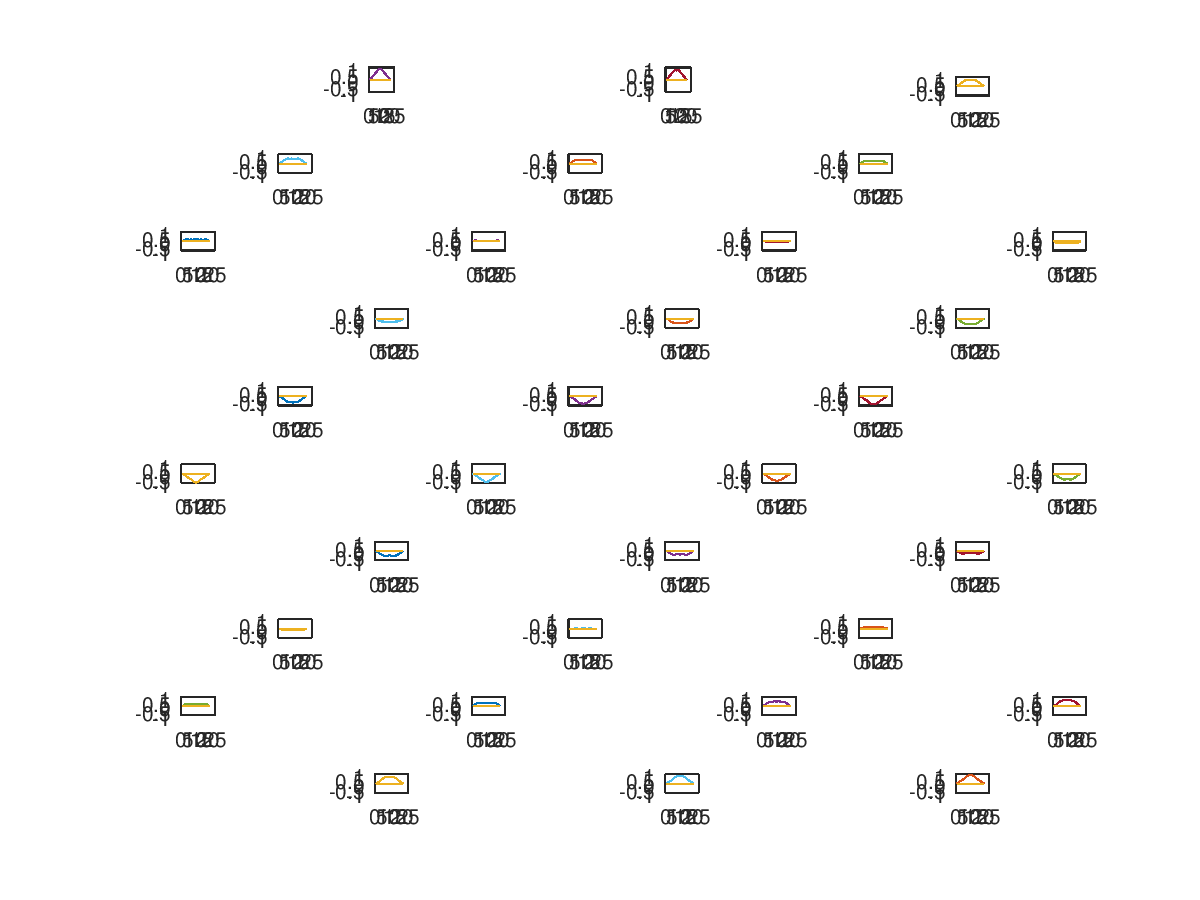
\includegraphics[width=\linewidth]{salida.png}
    \caption{Salida de imágenes paso a paso por partes}
    \label{fig:img_all}
\end{figure}
\begin{figure}[H]
    \centering
    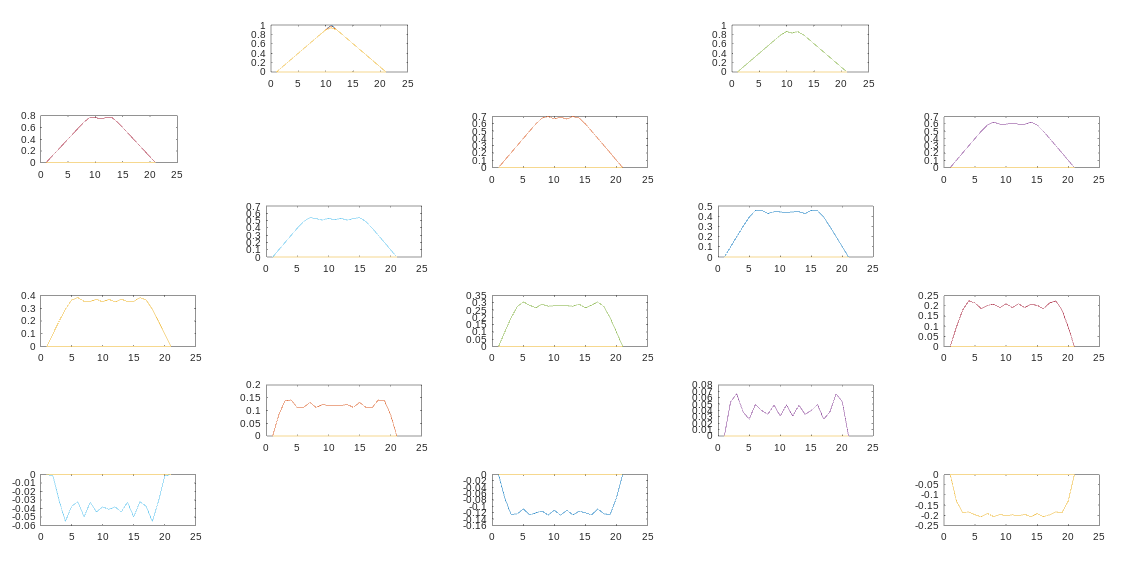
\includegraphics[width=\linewidth]{salida2.png}
    \caption{Salida de imágenes paso a paso escalada para visualizar mejor los resultados}
    \label{fig:img_all}
\end{figure}
\begin{figure}[H]
    \centering
    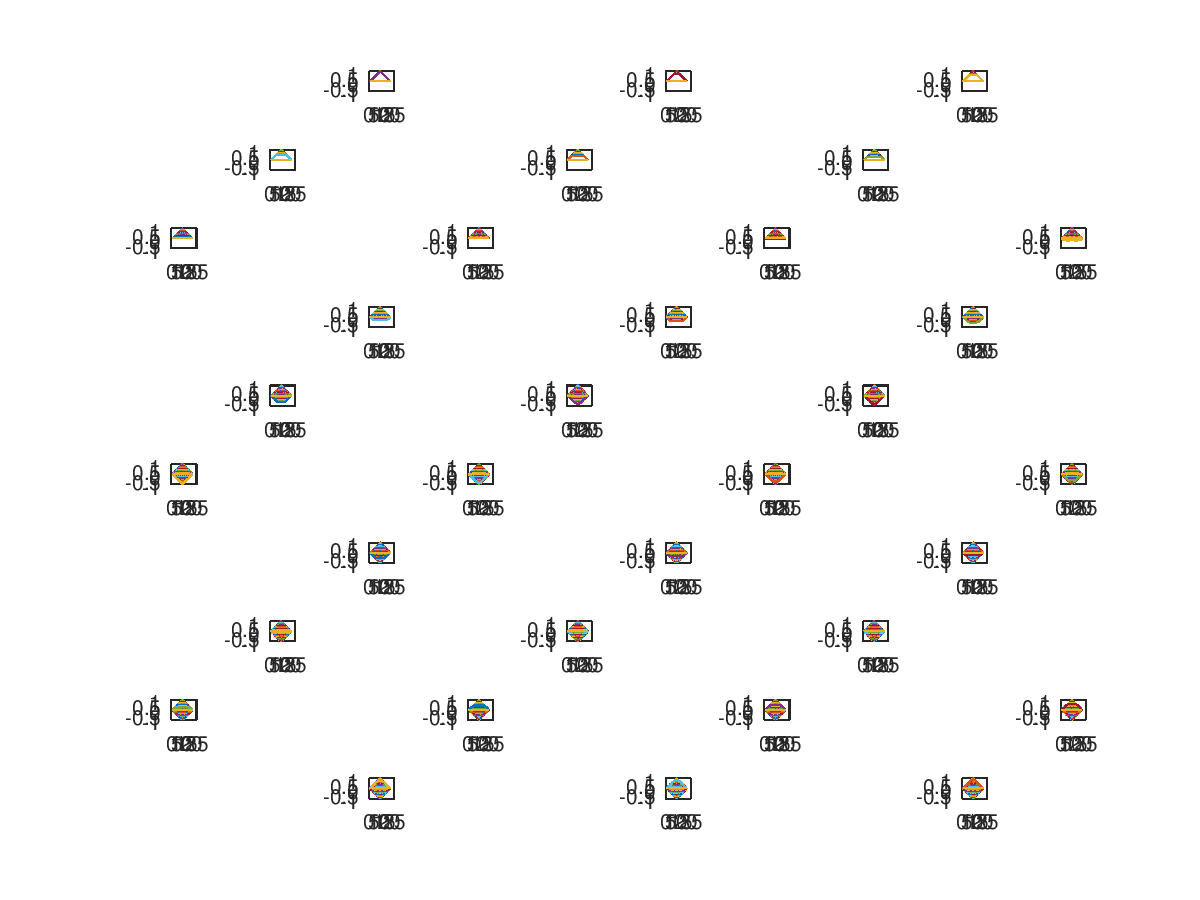
\includegraphics[width=\linewidth]{salida1.png}
    \caption{Salida de imágenes paso a paso por juntando las partes de los anteriores subplots}
    \label{fig:img_all}
\end{figure}

\end{document}
